\documentclass[fyp]{socreport}
\usepackage{bm}
\usepackage{fullpage}
\usepackage{url}
\usepackage{multirow}
\usepackage{graphicx}
\usepackage{amsthm}
\usepackage{amssymb}

\theoremstyle{definition}
\newtheorem{definition}{Definition}[section]
\theoremstyle{hypothesis}
\newtheorem{hypothesis}{Hypothesis}[section]

\begin{document}
\pagenumbering{roman}
\title{Leveraging Social Context in Fake News Detection with Graph Representation}
\author{Nguyen Van Hoang}
\projyear{2019/20}
\projnumber{H0791800}
\advisor{A/Prof. Min-Yen Kan, Dr. Kazunari Sugiyama}
\deliverables{
	\item Report: 1 Volume
	\item Source Code: 1 DVD}
\maketitle
\begin{abstract}
The popularity of social media in Web 2.0 has changed how the public shares and consumes news. The rapid dissemination of information allows both genuine and wrong news to reach millions of audiences within hours, impacting public opinions and decisions. In critical events such as pandemic responses or presidential elections, information factuality is an upmost concern in coordinating social behaviours and ensuring public fairness and rationality. Unfortunately, the tremendous volume and startling speed of news propagation renders manual fact-checking methods ineffective. Automatic approaches are mainly categorized into content-based models, which rely on the subject matter and its existing knowledge, and context-based models, which utilize social media perception towards the questionable news. While the former arguably gives explainable predictions, the latter makes few assumptions about the news content by utilizing the large and readily available wisdom of the crowd.

In this work, we propose Fake News Graph or FANG -- a novel graph-based social context representation and learning framework for fake news detection. We discuss its superiority in modeling social context as a graph compared with both content-based and Euclidean context-based baselines. Our approaches not only improves the macro performance of fake news detection but also obtains quality representations that generalize well to down-stream social network analysis. We observe consistent improvement across different data availability especially when given a limited training amount. Our recurrent aggregator accounts for temporal propagation patterns and enhances explainability with attention mechanism.

\begin{descriptors}
    \item C5 Computer System Implementation
	\item G2.2 Graph Algorithms
\end{descriptors}
\begin{keywords}
	Problem, algorithm, implementation
\end{keywords}
\begin{implement}
	Solaris 10, g++ 3.3, Tcl/Tk 8.4.7
\end{implement}

\end{abstract}

\begin{acknowledgement}
I am greatly thankful to have the guidance of Professor Min-Yen Kan, Dr. Kazunari Sugiyama, and recently Dr. Preslav Nakov. I would also like to extend my appreciation to Pan Liangming and Animesh Prasad, who are currently PhD candidates at NUS, for giving valuable research suggestions, as well as my fellows from NUS's Web IR / NLP Group (WING). I also like to thank Toshiki Tomihira, who was visiting WING as a research intern when I first started researching fake news, for many constructive discussion and collaboration.
\end{acknowledgement}

\listoffigures 
\listoftables
\tableofcontents 

\chapter{Introduction}
\label{ch:introduction}
\section{Background}
%Kaz: You do not need to insert space (~) just before "\footnote". 
% (But "~" is necessary for "\cite")
%Please also check other footnotes. 
There are two sides of Web 2.0. Social media connects billions of Internet users and is a conductive medium to spread information. The current speed of news dissemination is a great challenge to any effort to verify it as scale, and creates a risk of leaving falsehood unchecked. Fake news, as defined by its malicious intent~\cite{shu2017fake}, can be weaponized to distort public perception. Pizzagate conspiracy theory\footnote{\scriptsize{\url{https://en.wikipedia.org/wiki/Pizzagate_conspiracy_theory}}}, although debunked later, went viral during the 2016 United States presidential election, wrongfully tarnished the reputation of some candidates and benefited others. 
%Kaz: ``...'' (correct double quotation mark in Latex not "...")
%Please also check the other sections.  
The popularity of the term ``fake news'' gave itself the title ``word of the year'' by American Dialect Society\footnote{\scriptsize{\url{https://time.com/5091268/fake-news-word-of-the-year/}}}.

Recent research by MIT~\cite{vosoughi2018spread} confirms that fake news reaches 1,500 people 6 times faster than true stores. and is 70 more likely to be retweeted. To make matter worse, modern recommendation systems and social networks personalize user news feed and suggest connections based on preference for existing narratives, such as vaccination~\cite{ludolph2016manipulating}. These groups of online users form echo chambers~\cite{quattrociocchi2016echo}, and amplify the propagation of news by confirming their bias. 
%Kaz: "Fake news identification" is better than "fake news discrimination"?  
%Fake news discrimination 
Fake news identification is a non-trivial task. Although general public are confident in their ability to discriminate false information, recent studies have shown the exact opposite. 39\% of Americans claim to be "very confident" and an extra 45\% to be "somewhat confident" in recognizing fake news, however, 75\% of them view a false story as accurate despite having seen it~\cite{edkins_2016}. Another study conducted in Singapore shows that 90\% of the subjects falsely believe in at least one out of five fake headlines, even though four out of five Singaporeans claim that they can confidently spot fake news~\cite{ng_2018}. As fake news is written with the intention to mislead readers, inferring news veracity solely based on its content is challenging~\cite{shu2017fake}. Many sites and social media have devoted great effort in identifying false information. Facebook encourages user to report non-credible posts~\footnote{\scriptsize{\url{https://www.facebook.com/help/572838089565953?helpref=faq_content}}}, them it employs expert analysis to expose or confirm questionable stories. This method is also used by fact-checking websites such as Snopes\footnote{\scriptsize{\url{snope.com}}} or Politifact\footnote{\scriptsize{\url{politifact.com}}}. With the ever-increasing amount of information, automated news verification systems consider external knowledge databases as evidences~\cite{hassan2017claimbuster}~\cite{thorne2017extensible} to verify controversial claims. 

\section{The Problem}
Fact-checking or content-based models achieve high accuracy, but often takes human resources and time to collect and process sufficient evidences, during which false information might have spread and caused severe damage. Recent research direction 
%Kaz: It is better to specify both official name and its abbreviation. 
% In addition, although "FND" first defined in "Abstract", it is better to define it 
% again when new section begins.   
%in FND
in fake news detection (FND) takes another turn and explores various features of the news dissemination process. Our observations show that there is a distinctive engagement pattern of social user towards fake and real news. 
%Kaz: table => Table
%Please also check other sections. 
The fake news example in Table~\ref{table:temporal_engagement_fake} has a large number of engagements within a short amount of time right after its publication. These engagements are mainly verbatim reports or negative comments explained by the typically appalling contents of fake news. After that short window we begin to see denial comments questioning the validity of the news, whereas the negative comments dwindles. The stance distribution stabilizes afterwards with no support or neutral comments. On the other hand, the real news example in Table~\ref{table:temporal_engagement_real} invokes moderate engagements mainly comprised of supportive and neutral comments, and the distribution of stance stabilizes quickly. Such temporal shift in user perception serves as an important signal in identifying false information. Many work has partly proposed a joint-representation of social context features as a network of social actors, whose links model various interactions of either stance expression between social users and news or following/follower relationships within social users~\cite{jin2014news}~\cite{gupta2012evaluating}\cite{popat2017truth}~\cite{shu2019beyond}. However, no works have comprehensively proposed a joint of medium of all major social entities, i.e., questionable news, media source, and social users, and their interactions. 

\begin{figure}[t]
\centering
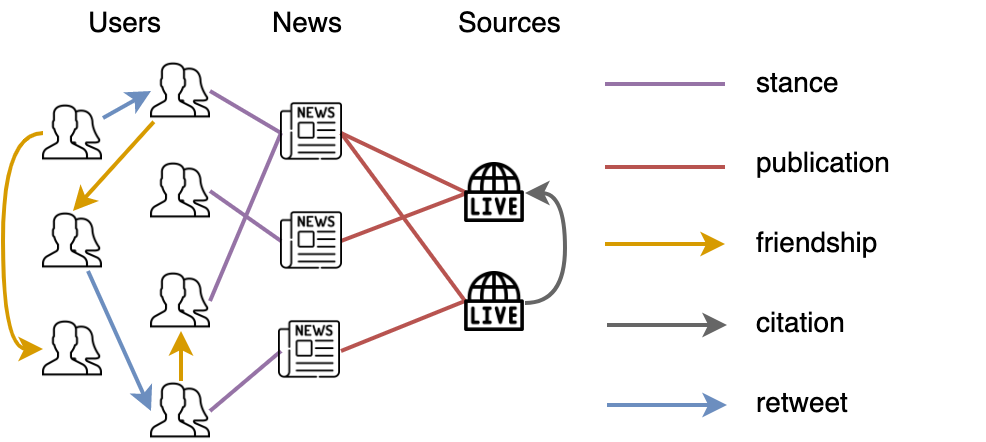
\includegraphics[scale=0.5]{social_graph_final.png}
\caption{Graph Representation of Social Context}
\label{fig:social_graph}
\end{figure}

\begin{table*}[t]
  \centering
  \tiny
  \begin{tabular}{|p{4cm}||p{1.5cm}|p{3cm}|p{5cm}|}
    \hline
    News title & Elapsed time - Total tweets  & Stance distribution - Support / Deny / Comment\_neutral / Comment\_negative / Report & Noticeable responses \\ \hline \hline
  Virginia Republican Wants Schools To Check Children's Genitals Before Using Bathroom & 3h - 38 & .00 / .03 / .03 / .16 / .78 & "DISGUSED SO TRASNPHOBIC", "FOR GODS SAKE  GET REAL GOP", "You cant make this up folks" \\ \cline{2-4}
  & (3h - 6h) - 21 & .00 / .10 / .05 / .05 / .80 & "Ok This cant be real", "WTF IS THIS BS", "Rediculous RT" \\ \cline{2-4}
  & $>$ 6h - 31 & .00 / .10 / .07 / .07 / .76 & "Cant make this shit up", "how is this real", "small government", "GOP Cray Cray  Occupy Democrats" \\ \hline
  \end{tabular}
  \caption{Temporal engagement of social users towards fake news}
  \label{table:temporal_engagement_fake}
\end{table*}

\begin{table*}[t]
  \centering
  \tiny
  \begin{tabular}{|p{4cm}||p{1.5cm}|p{3cm}|p{5cm}|}
    \hline
    News title & Elapsed time - Total tweets  & Stance distribution - Support / Deny / Comment\_neutral / Comment\_negative / Report & Noticeable responses \\ \hline \hline
  1,100,000 people have been killed by guns in the U.S.A. since John Lennon was shot and killed on December 8, 1980 & 3h - 9 & .56 / .00 / .00 / .00 / .44 & "\#StopGunViolence", "guns r the problem" \\ \cline{2-4}
  & $>$ 3h - 36 & .50 / .00 / .11 / .00 / .39 & "Some 1.15 million people have been killed by firearms in the United States since Lennon was gunned down", "\#StopGunViolence" \\ \hline
  \end{tabular}
  \caption{Temporal engagement of social users towards real news}
  \label{table:temporal_engagement_real}
\end{table*}

\section{Our Solution}
Social context of news dissemination is inherently represented as a heterogeneous graph whose nodes are the social entities and their auxiliary features, and whose edges are the social interactions. A graph medium has several advantages over some existing Euclidean-based methods~\cite{ruchansky2017csi}~\cite{liu2018early} in terms of structural modeling capability for several phenomena like filtering bubbles of users or polarized network of news media. Network modelling also allows entities to exchange information, via homogeneous edges, i.e., user-user relationship, source-source citations, heterogeneous edges, i.e., user-news stance expression, source-news publication, and high order proximity, i.e., between users who consistently support or deny certain sources, which are illustrated in  
%Such illustration is described in Figure~\ref{fig:social_graph}. 
Figure~\ref{fig:social_graph}.  
Previous attempts to learn such structure have employed spectral-based approaches ~\cite{shu2019beyond}~\cite{gupta2012evaluating}, whose expensive matrix factorization lacks consideration for higher order proximity, and whose representations are highly specific to the discussed task. Furthermore, there has been no in-depth analysis of the learned embeddings and their correlation to underlying communities.

%Kaz: You can write like "Fake News Graph (FANG)" 
%We propose Fake News Graph or FANG, 
We propose Fake News Graph (FANG), a graph learning framework for the proposed network in both supervised and unsupervised settings. FANG explores new information sources by looking at the context of news spreading pattern and temporality. FANG models the social actors (news, sources, users) under a common medium that accounts for their interaction, and utilizes recent advancements in Graph Neural Network (GNN)~\cite{kipf2016semi}~\cite{grover2016node2vec}. Given a joint representation space of social actors, we examine if separate node classification tasks, i.e., troll detection for users, FND for news, bias/factuality detection for sources, can benefit from a supervised multi-task learning objective, or unsupervised pre-trained context-aware embedding. FANG outperforms Euclidean baseline on the task of FND and achieves competitive performance given limited labels. We also analyze how the learned structural representations of social actors correlate with their underlying communities such as echo chambers of users or polarized networks of media, and how robust they are to various downstream tasks.

Our major contributions are summarized as follows:
\begin{enumerate}
    \item We provide a novel graph representation for the social context of news dissemination, which models all major social actors and interactions.
    \item We propose FANG, a novel graph learning framework that explores the unique structures of social context graph in both supervised and unsupervised settings.
    \item We conduct extensive experiments to assess the performance of FANG in FND and its produced structural representations on downstream classification tasks of social entities.
\end{enumerate}

%\section{Report Organization}
\section{Structure of Our Report}
%The structure of this report is organized as
This report is organized as follows: 
\begin{itemize}
    \item In Chapter 1, we introduce the problem of fake news, motivate the exploration of social context and present our solution of a novel graph representation and learning framework.
    \item In Chapter 2, we review the related literature in the domain of FND and graph learning frameworks.
    \item In Chapter 3, we formalize the problems of representing social context and detecting fake news. We describe the proposed methodology to address the problems in details.
    \item In Chapter 4, we evaluate our proposed solution by analyzing the experimental results.
    \item In Chapter 5, we conclude the report with a discussion on future research directions.
\end{itemize}
%As the an on-going research, 
As our work is ongoing, some aspects of the problem have not been discussed yet and will be revisited in later reports. 


\chapter{Related Work}
\label{ch:related}

We review existing works on representation learning frameworks of social context, specifically euclidean-based and network-based, which are more relevant to our research. We also discuss the recent advancement in Geometric Deep Learning framework, and how they can be applied to our social context graph. Here, we highlight the advantages and disadvantages of different methods, and motivate the choice of our solution.

Euclidean-based approaches seek to incorporate social context by extracting features of media or users who spread the news and combining those with content-based features~\cite{castillo2011information}~\cite{yang2012automatic}. User features at individual-level~\cite{shu2017fake} consider both attributes such as demographics, information preferences, social activeness, and network structure such as follower or friend counts, which do not reveal much about each user's neighborhood other than his centrality. Even at group-level, user features are merely the aggregation of individual-level features like ``average number of users''~\cite{ma2015detect}. Such representations are relatively easy to construct and analyzed but completely lack the modelling capability for users from a common community. Furthermore, users can engage to a piece of news in different ways by expressing different stances or sentiments via various temporal patterns, which was not considered in these early works.

Networks in which nodes constantly exchange and propagate information such as trust~\cite{kamvar2003eigentrust} or any auxiliary attributes~\cite{liao2018attributed} have been widely discussed. Recent works in detection falsehood has generalize the idea to social context by modelling an underlying user or news source network and dedicate a representation that captures an entity's structural features. CSI~\cite{ruchansky2017csi} used linear dimensionality reduction on user co-sharing adjacency matrix and combine it with the news engagement feature obtained from a recurrent neural network. TriFN~\cite{shu2019beyond}, which might seem similar to our proposal, neither differentiated user engagements in term of stance and temporal patterns, nor modeled source-source citation. Furthermore, such matrix decomposition approaches, including CSI~\cite{ruchansky2017csi}, are potential expensive in term of graph node counts and ineffective in modeling high-order proximity. Other works on citation source network~\cite{kulkarni2018multi}, propagation network~\cite{monti2019fake}, rumor detection~\cite{yuan2019jointly} utilized recent advances in graph neural network and multi-head attention attention to learn both local and global structural representation. However, the authors neither considered a comprehensive social context graph, nor presented any study for the embedding expressiveness for underlying social structures such as echo chambers or polarized media networks, probably due to an incomplete graph representation.

\begin{table*}[t]
  \centering
  \tiny
  \begin{tabular}{|p{4cm}|p{2.5cm}|p{4cm}|p{1cm}|p{2cm}|p{1cm}|}
    \hline
    Approach & Category & Modeled social entities \& interactions & Temporal & Learning Framework & Structural Expressiveness \\ \hline \hline
    Castillo (2011)~\cite{castillo2011information}, Yang (2012), Ma (2015)~\cite{ma2015detect}~\cite{yang2012automatic} & Feature-based model & Users, News & No & Euclidean-based learning & No \\ \hline
    CSI~\cite{ruchansky2017csi} & Graph representation \& Euclidean learning & User, News, User-user followership, User-news interaction & Yes & Matrix factorization, Recurrent Neural Network & No \\ \hline
    TriFN~\cite{shu2019beyond} & End-to-end Graph & User, News, Sources, User-user followership, User-news interaction, Source-news publication & No & Matrix factorization & No \\ \hline
    Kulkarni (2018)~\cite{kulkarni2018multi} & Graph representation \& Euclidean learning & News, Sources, Source-source citation, Source-news publication & No & GNN, Deep Network  & No \\ \hline
    Monti (2019)~\cite{monti2019fake} & End-to-end Graph & Users, News, User-user followership, User-news interaction & No & GNN & No \\ \hline
    GLAN~\cite{yuan2019jointly} & End-to-end Graph & Users, News, User-news interaction & No & GNN, Multi-head attention & No \\ \hline \hline
    FANG (this work) & End2end Graph (supervised), Graph representation \& Euclidean learning (unsupervised) & User, News, Sources, User-user followership, User-news interaction, Source-news publication, Source-source citation & Yes & GNN & Yes \\ \hline
    
  \end{tabular}
  \caption{Comparison between representation learning frameworks of social context}
  \label{table:literature_review}
\end{table*}
%Kaz: Did you define "GNN" before this paragraph/? 
Recent work in Graph Neural Network (GNN) have successfully generalize Deep Learning methods to learn both supervised and unsupervised representation of objects with complex relationships and interdependency. GCN~\cite{kipf2016semi} effectively approximate the parameters of convolutional filters in large graph. Other unsupervised approaches such as Node2Vec~\cite{grover2016node2vec} generalize distributed sampling to construct structural representation of graph nodes. Such spatial-based approaches using GNN have major advantages over spectral-based matrix factorization in term of modeling capacity for high-order proximity, edge-aware feature  propagation~\cite{velivckovic2017graph} and scalability in number of graph nodes.

%The comparison between the discussed works on representation learning frameworks of social context is summarized in Table~\ref{table:literature_review}
Table~\ref{table:literature_review} summarizes the comparison between the discussed works on representation learning frameworks of social context. 

\chapter{Problem and Algorithm}
In this chapter, we first formulate the problem of fake news detection, and our research hypothesis. We then discuss the construction of social context graph, including feature extraction of each social entities and edge interaction labelling. We will describe the methodology of FANG in details as well as the intuition behind it.

\section{Fake News Detection from Social Context}
To ensure a consistent representation, let us first define social context, formulate the task of context-FND and formalize our research hypothesis. The fundamental entities and interactions of the social context $C$ are described as follows: 
\begin{enumerate}
    \item Let $A=\{a_1, a_2,...\}$ be the list of \textbf{news articles} that are being propagated through the social media. $a$ is defined by a feature vector $x_{a}$.
    \item Let $S=\{s_1, s_2,...\}$ be the list of \textbf{news sources} where each source $s_j$ has published at least one article in $A$. $s$ is defined by a feature vector $x_{s}$.
    \item Let $U=\{u_1, u_2,...\}$ be the list of \textbf{social users} where each user has engaged in spreading any article in $A$ or has a connection with any user in $U$. $u$ is defined by a feature vector $x_{u}$.
    \item Let $E=\{e_1, e_2,...\}$ be the list of interactions where each interaction $e=\{v_1, v_2, t, x_e\}$ describes an interaction between two entities $v_1, v_2\in A\cap S\cap U$ at time $t$, where $t$ can be absent in interactions that are time-insensitive. The interaction type of $e$ is defined as the label $x_{e}$.
\end{enumerate}
The characteristics of each interaction is further described in Table~\ref{table:social_interactions} and illustrated in Figure~\ref{fig:social_graph}.

\begin{table*}[t]
  \centering
  \tiny
  \begin{tabular}{|p{1.5cm}|p{2cm}|p{2.5cm}|p{5cm}|p{1cm}|}
    \hline
    Interaction & Linking entities & Linking type & Description & Time-sensitive \\ \hline \hline
    Followership & User-user & Unweighted, directed & Following/follower relationship on mainstream social media & No \\ \hline
    Citation & Source-source & Unweighted, directed & The percentage of reference hyperlink between one media source to another & No \\ \hline
    Publication & Source-news & Unweighted, undirected & The relationship between a media source and its published articles & Yes \\ \hline
    Stance & User-news & Multi-label, undirected & The perception of social users towards a news article & Yes \\ \hline
    Retweet & User-user & Unweighted, directed & The propagation of information from one user towards another & Yes \\ \hline 
  \end{tabular}
  \caption{Interactions in social context}
  \label{table:social_interactions}
\end{table*}

%Kaz: i.e. => I.e.*,*
Publication, stance and retweets are special types of interaction as it is not only characterized by its spatial features, i.e., edge labels, source/destination nodes, but also by its temporal features, i.e., when the interactions happen. Recent works have highlighted the importance of incorporating temporality in modeling social context engagement, not only in fake news detection~\cite{ruchansky2017csi}~\cite{ma2015detect}, but also in modeling online information dissemination~\cite{he2014predicting}. In this work, we are using six  stance labels, namely \textit{support}, \textit{deny}, \textit{negative\_comment}, \textit{neutral\_comment}, \textit{unrelated}, \textit{report}. Four of our stance labels, \textit{support}, \textit{deny}, \textit{comment}, \textit{unrelated} are consistent with the recent work on stance detection~\cite{mohtarami2018automatic}. Based on our observation of the distinguished sentiment of engagement towards fake and real news in Chapter~\ref{ch:introduction}, we classify \textit{comment} further into \textit{negative\_comment} and \textit{neutral\_comment}. We assign the ``report'' stance label to an user-news engagement when the user simply propagates the news article without expressing any opinion. Altogether, stances are used to characterize news articles by their perceived public opinions, as well as social users by their view on different journalism content. Table~\ref{table:stance_examples} shows examples for different stances.

\begin{table*}[t]
  \centering
  \tiny
  \begin{tabular}{|p{4cm}|p{7cm}|p{2cm}|}
  \hline
    News title & Tweet & Stance \\ \hline \hline
  US Representatives Agree To Illicit UN Gun Control Plans & More proof we should pull out of the UN and throw them out of the US Pot us Real Donald Trump US Representative & support \\ \cline{2-3}
  & This can't be right & deny \\ \cline{2-3}
  & Oh my giddy aunt & neutral\_comment \\ \hline
  Pence Michelle Obama Is The Most Vulgar First Lady We've Ever Had & How dare you sir that's our First Lady respect Pence Michelle Obama Is The Most Vulgar First Lady We've Ever Had & negative\_comment \\ \cline{2-3}
  & RT Janice GW Pence Michelle Obama Is The Most Vulgar First Lady We've Ever Had USA Newsflash & report \\ \cline{2-3}
  & Lawrence run with this PLEASE & unrelated \\ \hline
  \end{tabular}
  \caption{Examples of user stances towards news articles}
  \label{table:stance_examples}
\end{table*}

We refer to the definition of general FND by Kaishu~\cite{shu2017fake} and formally define the task of context-based FND.
\begin{definition}{\textit{Context-Based FND}}: Given a social context $C(A,S,U,E)$ constructed from news articles $A$, news sources $S$, social users $U$, and social interactions $E$,
%Kaz: Can you rephrase "Context-based Fake News Detection" to "Context-based FND" as FND is used in the previous part. 
%Hoang: Thank you, I have rephrased.
Context-based FND is defined as the binary classification task of predicting whether a news article $a\in A$ is fake or not, i.e.,  $F_C : a \rightarrow \{0,1\}$ such that,
\[  F_C(a) = \left\{
\begin{array}{ll}
      0 & \textrm{if } a \textrm{ is a fake article} \\
      1 & \textrm{otherwise} \\
\end{array} 
\right. \]
\end{definition}
Context-based FND is considered a semi-supervised learning problem where we train our classifier on the partially labelled articles to approximate $F_C$ and predict whether the unlabeled articles are fake or not.
\begin{hypothesis}Given a social context $C(A,S,U,E)$, we hypothesize that our graph representation and learning framework, i.e., FANG, improve the structural features of social actors $A,S,U$, resulting in more accurate fake news detection.
\end{hypothesis}

\section{Graph Construction from Social Context}
\label{sec:graph}
In this section, 
%Kaz: Rephrased the following phrase. You can use "detail"  as a verb. 
%we describe details 
we detail our social context graph construction. We specify the selected features for each social entities, i.e., $x_a$, $x_s$, $x_u$, and how we obtain the labels for each social interaction, i.e., $x_e$.

\textbf{News Articles}: News content is a major component in detecting the authenticity of the news itself. Textual~\cite{castillo2011information}~\cite{yang2012automatic}~\cite{shu2019beyond}~\cite{popat2018credeye} and visual~\cite{wang2018eann}~\cite{khattar2019mvae} have been widely used to model news article contents, either by feature extraction, unsupervised semantics encoding, or learned representation. In this work, we are looking at unsupervised semantics encoding as it is relatively efficient to construct and optimize. We are aware of non-end-to-end limitation and would like to leave this as an open research question.

In the scope of this report, we consider only textual features. For each article $a\in A$, we constructed the tf-idf~\cite{sparck2004idf} vector $v^t_a$ from text body in the article. We increase the semantics expressiveness of token-based representation by weighting them with pre-trained word embeddings obtained from GloVe~\cite{pennington2014glove} to obtain $v^s_a$. The news article feature vector $x_a$ is created by concatenating $v^t_a$ and $v^s_a$.

\textbf{News Sources}: Characteristics of media sources that publishes the questionable news have been widely adopted as a essential indicator of the news trustworthy~\cite{baly2018predicting}~\cite{kulkarni2018multi}. Commonly utilized features include journalism topics, lexicon-derived bias, url structure and social network trace~\cite{baly2018predicting}. This report focuses mainly on characterizing media sources by their reporting textual content. For each source $s$, similar to article representations, we constructed the source feature vector $x_s$ 
%Kaz: You can just describe "tf-idf vector" not "a bag-of-word tf-idf vector" as we often use a "bag-of-word vector". 
as the concatenation of a bag-of-word tf-idf vector $v^t_s$ and a semantics-sensitive vector $v^s_s$ derive from the ``homepage'' and ``about-us'' directory. A portion of fake news spreading websites give a ``disclaimer'' of being a satirical or sarcastic media in the their ``about-us'' --- a helpful signal for the journalism quality. 

\textbf{Social Users}: Online users have been studied extensively as the major propagator of fake news and rumors in social media. As discussed in chapter~\ref{ch:related}, previous work~\cite{castillo2011information}~\cite{yang2012automatic} utilized attributes  such  as  demographics,  information  preferences,  social activeness, and network structure such as follower or friend counts. A recent work by Kai Shu~\cite{shu2019role} conducted a feature analysis on user profile and pointed out the importance of signals derived from profile description and timeline content. A text description such as "American mom fed up with anti american leftists and corruption. I believe in US constitution, free enterprise, strong military and Donald Trump \#maga" strongly indicates the user political bias and suggest the tendency to promote certain narratives. We calculate the user vector $x_u$ as the concatenation of a pair of tf-idf vector $v^t_u$ and semantics vector $v^s_u$ derived from the user profile text description.

\textbf{Social interactions}: For every social actor pairs $(v_i, v_j)\in A\cap S\cap U$, we add an edge $e=\{v_i, v_j, t, x_e\}$ to the list of social interactions $E$ if they interact via interaction type $x_e$. Specifically, for followership, we examine if user $u_i$ follows user $u_j$ on social media; for publication, we examine if news $a_i$ was published by source $s_j$; for retweet, we examine if user $u_i$ has ever retweeted user $u_j$; for citation, we examine if the homepage of source $s_i$ contains any hyperlink to source $s_j$. In the case of time-sensitive interactions, i.e. \textit{publication}, \textit{retweet} and \textit{stance}, we record their relative timestamp with respect to the article's earliest publication time. 

\textbf{Stance detection}: The task of obtaining the correct type for each \textit{stance} interaction is formulated as \textit{stance detection}. Given the large number of user-news interactions and the limited amount of annotation in current social context data, we train a stance classification model. Although the labeled data for tweet stance classification is limited, the abundance of labeled data for stance classification on general news~\cite{hanselowski2018retrospective} and tweet pair classification~\cite{xu-etal-2015-semeval} inspires us to conduct Transfer Learning (TL)~\cite{pan2009survey}. The TL architecture is described in figure~\ref{fig:transfer_learning}. Notice that this is a cross-corpus, i.e. from general news to tweets, and cross-task, i.e. from tweet paraphrase identification to stance detection, TL.

\begin{figure}[t]
\centering
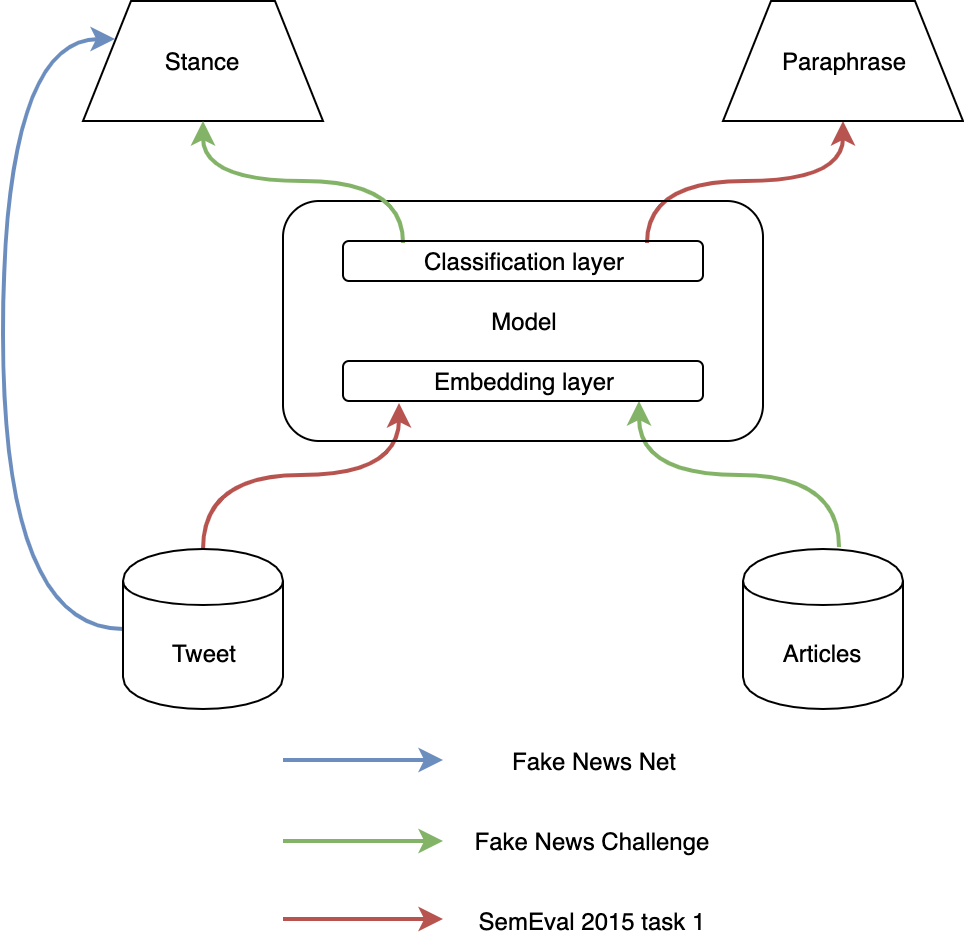
\includegraphics[scale=0.3]{transfer_learning.png}
\caption{Cross-corpus, cross-task TL for stance detection}
\label{fig:transfer_learning}
\end{figure}

The first model is trained on tweet corpus with the objective to detect if two input tweets are paraphrases, while the second model is trained on news article corpus with the objective to detect the stance of an article's body towards its headline~\cite{hanselowski2018retrospective}. The final stance detection model is trained on a limited amount of annotated tweet pairs with stance labels from FakeNewsNet~\cite{shu2018fakenewsnet} of 2110 samples of 474 supports, 298 denies, 387 comments and 951 unrelated tweets. This model is trained with using the embedding layer initialized with the first model's pretrained weights and the classification layer initialized with the second model's pretrained weights. We choose BiDAF~\cite{seo2016bidirectional} for our classifier as it is a light-weight deep learning model to learn the mutually attentive representations of two input sentences. Experiment results in table~\ref{table:stance_results} show that our TL BiDAF reached 0.9 macro F1 and manage to improves state-of-the-art pretrained BERT-based~\cite{devlin2019bert} language models by 31.8\% macro F1 error rate. For each user-news interaction $e=(u_i, a_j, t, x_e)$ at time $t$, we input the tweet text and news article's title into our stance detection model to obtain the stance label $x_e$. We also finetune a pre-trained Roberta model~\cite{liu2019roberta} on Stanford Sentiment Treebank\footnote{\scriptsize{\url{https://nlp.stanford.edu/sentiment/treebank.html}}} to obtain a sentiment classifier and differentiate \textit{neutral} and \textit{negative} comments.

\begin{table*}[t]
  \centering
  \tiny
  \begin{tabular}{|p{6cm}|p{2cm}|p{2cm}|p{2cm}|p{2cm}|}
  \hline
    Model & Accuracy & Precision & Recall & Macro F1 \\ \hline \hline
    BiDAF & 0.8657 & 0.8558 & 0.8454 & 0.8465 \\ \hline
    Bert-base-uncased~\cite{devlin2019bert} & 0.8458 & 0.8153 & 0.8248 & 0.8194 \\ \hline
    XLNet-base-cased~\cite{yang2019xlnet} & 0.8308 & 0.7986 & 0.8004 & 0.7976 \\ \hline
    XLM~\cite{lample2019cross} & 0.8109 & 0.7806 & 0.7835 & 0.7817 \\ \hline
    Roberta-base~\cite{liu2019roberta} & 0.8806 &	0.8545 & 0.8678 & 0.8588 \\ \hline \hline
    \textbf{TL BiDAF} & \textbf{0.9154} & \textbf{0.9059} & \textbf{0.9032} & \textbf{0.9037} \\ \hline
  \end{tabular}
  \caption{Stance Detection Results}
  \label{table:stance_results}
\end{table*}

\section{FANG}
\label{sec:fang}
In this section, we discuss the our current research progress on Time-insensitive supervised FANG --- the proposed Graph Learning Framework in supervised learning without considering temporality. We will discuss the potential research for time-sensitive supervised FANG, as well as unsupervised FANG in section~\ref{sec:future_work}.

\textbf{Time-insensitive Graph Neural Network baseline}: Inspired by the recent advancement of Graph Convolutional Networks (GCN)~\cite{kipf2016semi}, we propose a baseline GCN-FANG which is a direct application of GCN to our proposed graph representation. Let the total number of social entities to be $N=|A|+|S|+|U|$. Each relation $r_k$ amongst our ten relations (four non-stance relations and six stances) is represented as a binary adjacency matrix $M_k\in \mathbb{R}^{N\times N} $ such that 
\[  M^{(ij)}_k = \left\{
\begin{array}{ll}
      1 & \textrm{if their is $r_k$ relation between the \textit{i}th and the \textit{j}th social actor} \\
      0 & \textrm{otherwise} \\
\end{array} 
\right. \]

where $M^{(ij)}_k$ is the element at $i$th row and $j$th column of $M_k$.

In consistent with the original paper, we define $X\in \mathbb{R}^{N\times d_1}$ to be the input node feature matrix where $X^{(i)}\in \mathbb{R}^{d_1}$ is the feature vector of $i$th social actor defined in section~\ref{sec:graph}. Let $d_l$ be the size of any node hidden representation obtained at the $l$th layer of GCN-FANG. We define the convolution operation in our graph consisting of multi-label edges as

\begin{equation}
    H_{l+1} = \parallel^{K}_{k=1}(\tilde{D}^{-\frac{1}{2}}\tilde{M}_k\tilde{D}^{-\frac{1}{2}}H_l\Theta_l)
\end{equation}

where $H_l\in \mathbb{R}^{N\times d_l}$ is the hidden representation matrix of social actors at $l$th layer, $\parallel$ is the concatenation operation, $K=10$ is the number of relations, $\Theta\in\mathbb{R}^{d_l\times d_{l+1}}$ is the matrix of optimizable weights at $l$th layer, and $\tilde{D}^{-\frac{1}{2}}\tilde{M}_k\tilde{D}^{-\frac{1}{2}}$ is the computation to obtain normalized graph Laplacian matrix. Notice that $H_1=X$ is the input feature matrix. After L layers, we obtain the output vector as the final hidden representation of each article $a$, or $\boldsymbol{o_a}=H^{(\bar{a})}_L$ where $\bar{a}$ is the index of $a$. $\boldsymbol{o_a}$ is passed through a softmax activation function $\sigma$, and all learnable weights are trained using cross-entropy loss as defined by $\mathcal{L}$:

\begin{equation}\label{eq:overall_loss}
    \mathcal{L}=\frac{1}{|A_c|}\sum^{A_c}_{a}\boldsymbol{y}_{a} \cdot log(\sigma(\boldsymbol{o}_{a}))+(1-\boldsymbol{y}_{a})\cdot log(1-\sigma(\boldsymbol{o}_{a}))
\end{equation}

where $A_c$ is a subset of labeled news articles where the label of each article $a$ is denoted as a one-hot encoded $\boldsymbol{y}_{a}\in \{0, 1\}^{2}$. The loss function is differentiable, thus trainable with Adam~\cite{kingma2014adam}.

\chapter{Evaluation}
In this section, we conducted experiments to evaluate the effectiveness of our proposed Graph Representation and Learning Framework. We will find answers to the following research questions:
\begin{enumerate}
    \item Do the proposed Graph Representation and Learning Framework work better than a euclidean representation baseline?
    \item Do the proposed Graph Representation and Learning Framework work well given limited training data?
    \item Do the proposed Graph Representation and Learning Framework given missing auxiliary features?
    \item Do the context-based models work better given temporal features?
\end{enumerate}

\section{Experiment Settings}
\textbf{Baselines}: To answer the first, third and fourth research question, we choose CSI~\cite{ruchansky2017csi} as our euclidean-based representation and learning baseline. We construct three variants
\begin{itemize}
    \item t-CSI where we retain the original model
    \item CSI where we remove the timestamp of social engagement
    \item f-CSI where we concatenate the user feature vector and source user vector obtained in section~\ref{sec:graph} to CSI's news article hidden representations
\end{itemize}

For our proposed GCN-FANG model, we also obtain two corresponding variants, GCN-FANG where we remove node features and f-GCN-FANG where we retain node features.

\textbf{Dataset}: The main dataset for this research is FakeNewsNet~\cite{shu2018fakenewsnet}, which contains the attributes and interactions of social actors. As the full dataset from Twitter is currently under retrieval, we extract a much smaller controlled dataset for experimentation which statistics are described in table~\ref{table:statistics}. The high sparsity of relation adjacency matrix provides both a limitation and opportunity for optimization.

\begin{table*}[t]
  \centering
  \tiny
  \begin{tabular}{|p{5cm}|p{5cm}|p{5cm}|}
  \hline
     & FakeNewsNet & Controlled \\ \hline \hline
    \#Users & 345440 & 2558 \\ \hline
    \#Sources & 566 & 35 \\ \hline
    \#News & 1056 (432 fake, 624 real) & 40 (20 fake, 20 real) \\ \hline
    \#Citation density & & 3\% \\ \hline
    \#Following density & & 0.003\% \\ \hline
    \#Stance density (support + deny) & & 2.5\% \\ \hline
  \end{tabular}
  \caption{Dataset statistics}
  \label{table:statistics}
\end{table*}

To answer the second question, we conducted experiments with different ratio of train/test and measured the classification metric of \textit{macro F1 score} on three baselines and two variants of our proposal. 

\section{Results \& Discussion}
The experiment results are described in table~\ref{table:experiment_results} and visualized in figure~\ref{fig:experiment_plot} and figure~\ref{fig:time_experiment_plot}.

\begin{table*}[t]
  \centering
  \tiny
  \begin{tabular}{|p{2cm}|p{2cm}|p{2cm}|p{2cm}|p{2cm}|p{2cm}|}
  \hline
     & f-GCN-FANG & GCN-FANG & f-CSI & CSI & t-CSI \\ \hline \hline
    0 & 1 & 1 & 1 & 1 & 1 \\ \hline
    0.1 & 1 & 1 & 1 & 0.6667 & 1 \\ \hline
    0.2 & 1 & 0.873 & 0.8889 & 0.6667 & 0.9091  \\ \hline
    0.3 & 1 & 0.8286 & 0.9091 & 0.6667 & 0.8 \\ \hline
    0.4 & 0.875 & 0.873 & 0.75 & 0.7692 & 0.7826 \\ \hline
    0.5 & 0.8 &	0.7494 & 0.9 & 0.5556 & 0.9474 \\ \hline
    0.6 & 0.873 & 0.703 & 0.8333 & 0.5455 & 0.75 \\ \hline
    0.7 & 0.9161 & 0.5942 &	0.75 & 0.5263 & 0.7333 \\ \hline
    0.8 & 0.8245 & 0.7163 & 0.6923 & 0.6667 & 0.7027 \\ \hline
    0.9 & 0.8381 & 0.6364 &	0.4653 & 0.381 & 0.6667 \\ \hline
    1 & 0 &	0 & 0 & 0 & 0 \\ \hline \hline
  \end{tabular}
  \caption{Experiment results}
  \label{table:experiment_results}
\end{table*}

\begin{figure}[t]
\centering
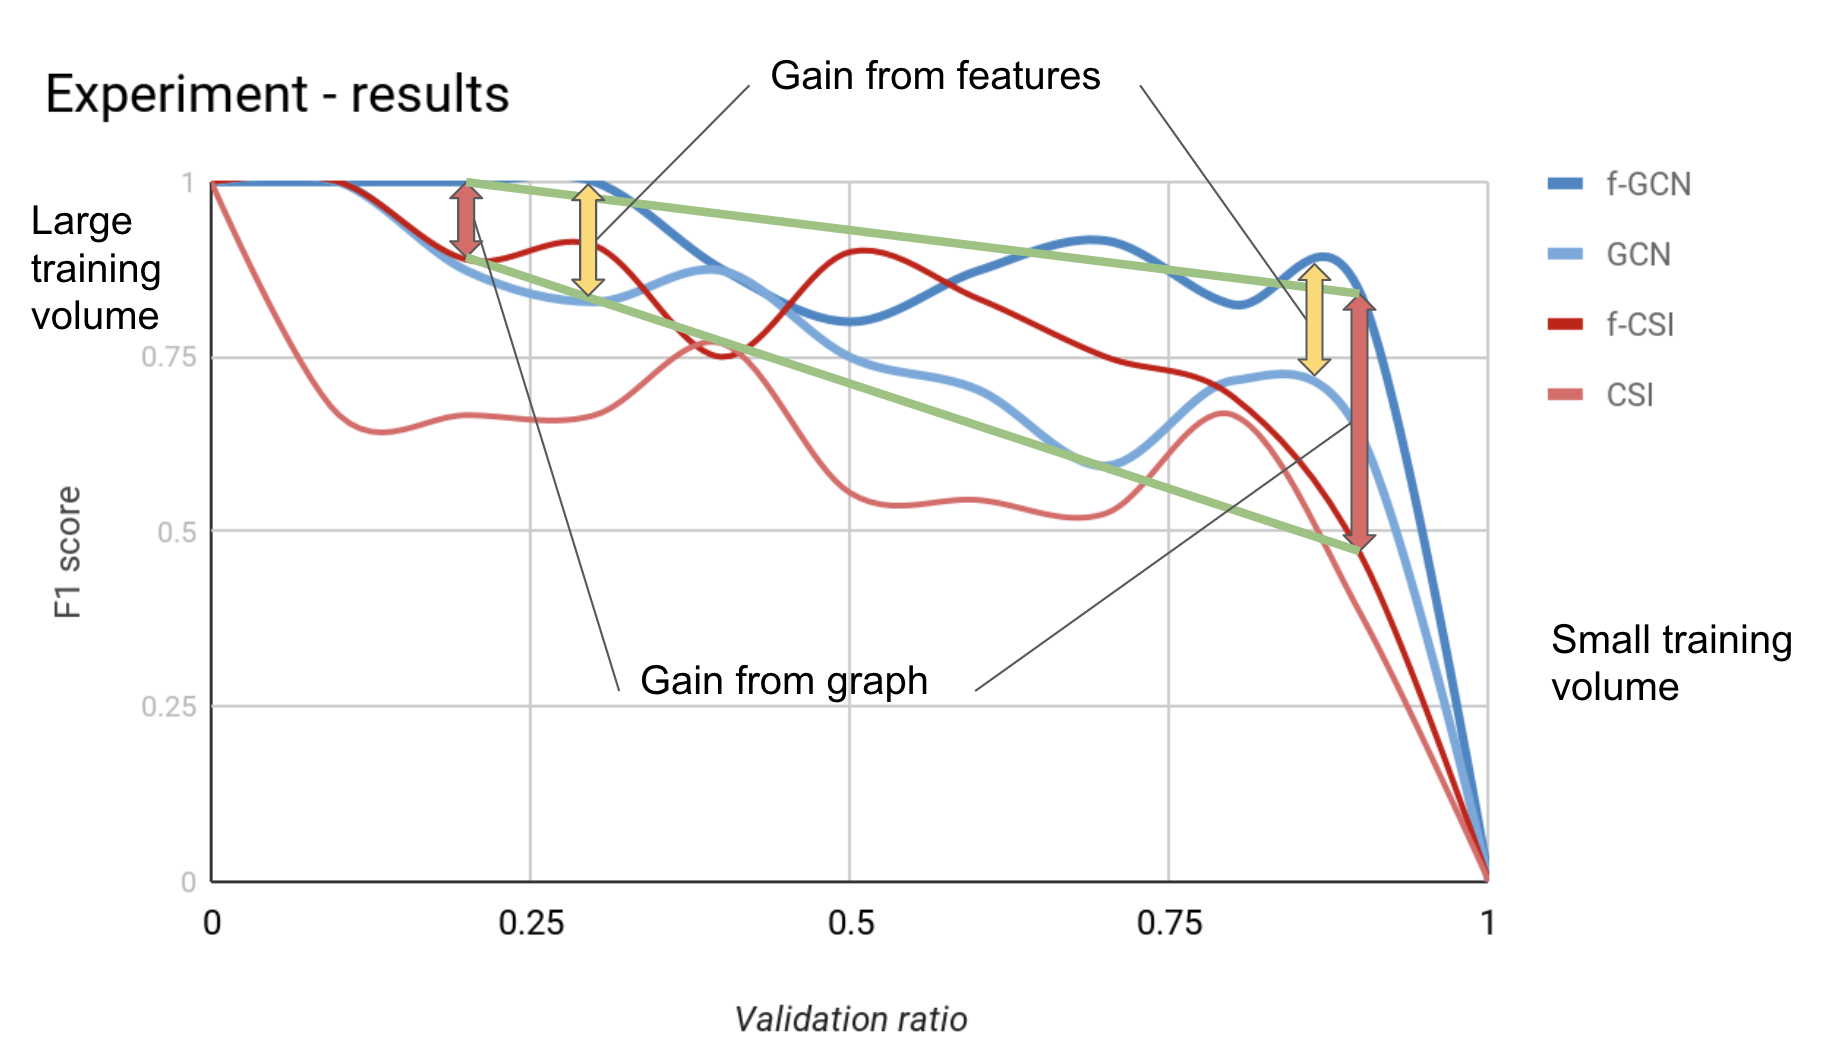
\includegraphics[scale=0.5]{experiment_plot.png}
\caption{Experiment result plot}
\label{fig:experiment_plot}
\end{figure}

\begin{figure}[t]
\centering
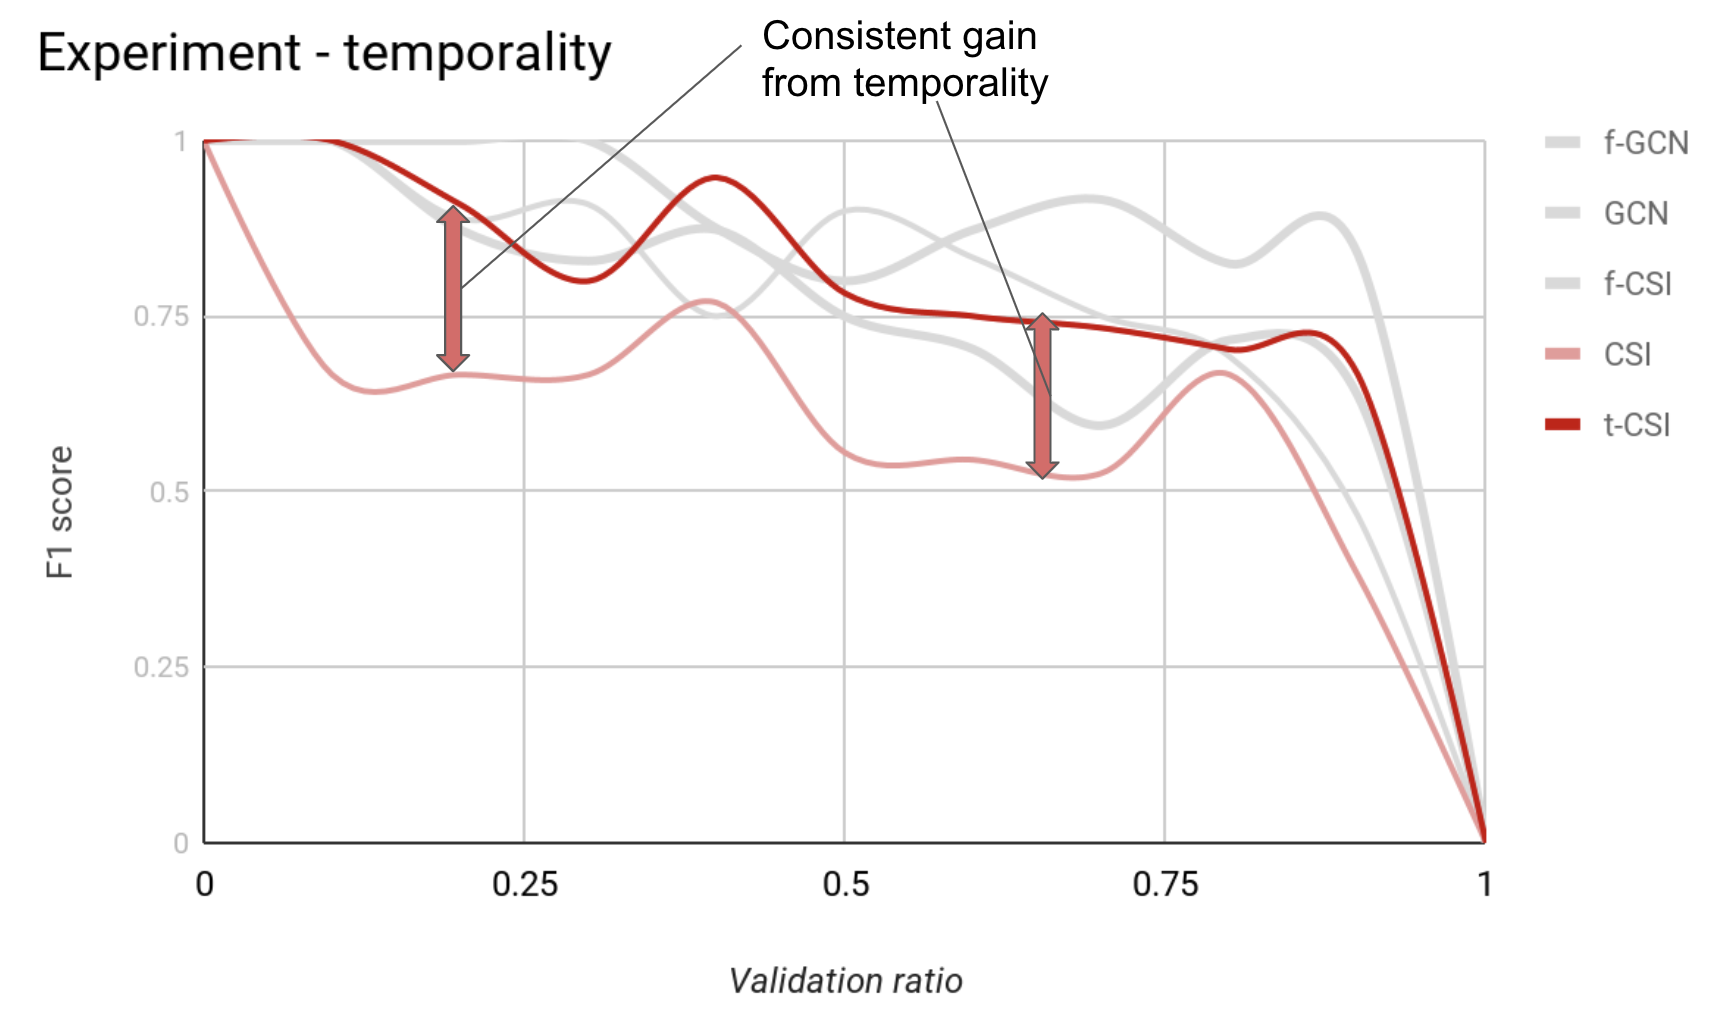
\includegraphics[scale=0.5]{time_experiment_plot.png}
\caption{Temporal experiment result plot}
\label{fig:time_experiment_plot}
\end{figure}

\textbf{Overall improvement}: We observe a consistent improvement from modeling social context as our proposed network structure. Both f-GCN-FANG and GCN-FANG outperform its euclidean-based CSI counterpart on almost all settings with different amount of data. The average improvement margins of F1 score are 10.42\% and 17\% respectively. This can be explained by the richer interactions and structural modeling at both local and global from graph-based approaches. 

\textbf{Limited training data}: Both the baselines and our proposed models perform worse when training data is limited. However, if we observe the performance when the validation ratios are 0.2 and 0.9, the gain for F1 score from FANG is much larger given the limited data, which are 11.11\% and 37.28\% respectively. This proves the robustness of our learning framework especially with limited training quantity.

\textbf{Limited or absent auxiliary features}: Both the baselines and our proposed models perform worse when node features are missing. However, the improvement margin for F1 score is greater between GCN-FANG and CSI, indicating that our proposed Graph Representation and Learning Framework excel at detecting fake news when social actors' attributes are absent or limited. The experiment results also emphasize the importance of incorporating auxiliary social features together with structural features to obtain the best performance.

\textbf{Temporality improvement}: Figure~\ref{fig:time_experiment_plot} highlights the improvement from incorporating temporal features to CSI baseline, which gives t-CSI a consistent and average improvement margin for F1 score of 20.53\%. This complies with our observation on the distinguished temporal engagement patterns between false and real news that can be utilized for fake news detection.

Overall, the experiment results confirm our research questions on the overall improvement, improvement given limited training data, improvement given absent auxiliary features and improvement given temporality.

\chapter{Conclusion}
\section{Contributions}
In this research report, we have addressed the importance of modeling social context of information propagation as graph. In addition to proposing a novel and comprehensive graph representation, we also described GCN-FANG, a graph learning framework based on GCN that shows consistent improvement over euclidean baseline in the task of fake news detection. We highlighted our greater gain in supervised learning settings of limited auxiliary features and limit training quantity, as well as the importance of incorporating temporal features in learning to represent social context.

\section{Future Work}
\label{sec:future_work}
This research is yet to complete. Before concluding this report, we would like to discuss several research direction that help us understand more about the manifold of social context and how we can derive intuitively representations of social entities that benefit various downstream tasks.

\textbf{Unsupervised or self-supervised FANG}: As mentioned in section~\ref{sec:fang}, we are looking forward to extending our current graph learning framework to unsupervised setting. The objective is to unsupervisedly capture a context-aware representation for each social entity that strongly correlates with underlying social communities such as echo chambers or polarized news network. One potential approach is an adaptation of neighborhood sampling scheme like Node2Vec~\cite{grover2016node2vec}, where the specific sampling strategy, i.e. which edge to traverse, walk length, context size, is different between social entities. A GNN-based auto-encoding approach, such as VGAE~\cite{kipf2016variational} can also be considered. We are also inspired by the recent breakthrough of pretrained language model with self-supervised objective~\cite{devlin2019bert}. A research direction is to structurally represent a node by predicting for readily available links in our networks such as stances.
Any unsupervised representation strategy for users that is stance-oriented can help us capture groups of users who share a common narrative, as illustrated in figure~\ref{fig:cluster}, which is an indication of echo chamber effect. Such unsupervised representation framework can also be time-sensitive and captures those who often engage in spreading a news article after a certain amount of time since publication. 

\begin{figure}[t]
\centering
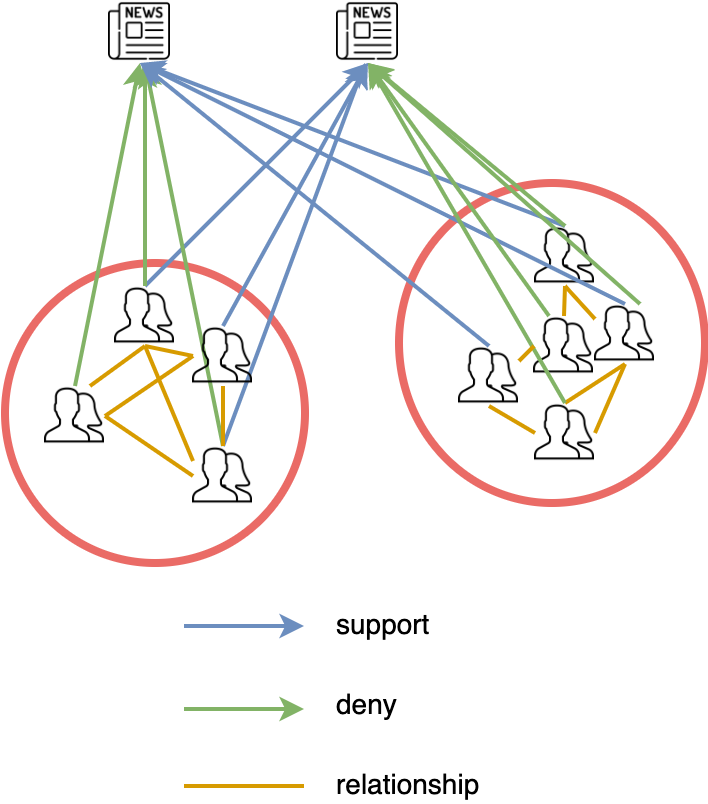
\includegraphics[scale=0.3]{cluster.png}
\caption{Underlying stance-based community}
\label{fig:cluster}
\end{figure}

\textbf{Mutli-task and multi-domain generalization}: Our graph provides a common medium for joint representations of heterogeneous social actors. Although we are examining fake news detection, any node classification task can benefit from our representation and learning framework, such as source bias and factuality prediction~\cite{baly2018predicting} or troll user detection~\cite{atanasov2019predicting}, either in a supervised setting with multi-task objective, or in an unsupervised setting by directly consuming our pretrained representations. We also realize that social context is a shared aspect in both fake news detection and rumor detection~\cite{zubiaga2018detection} and are looking forward to generalizing our approach to the other domain.

\bibliographystyle{socreport}
\bibliography{socreport}

\end{document}
